\newcommand{\specname}{SBCF}
\newcommand{\status}{Beta}
\newcommand{\ecn}{NA}
\newcommand{\revdate}{2013-03-16}
\newcommand{\rev}{000}
\newcommand{\relay}{PB2}
\newcommand{\boil}{PB3}
\newcommand{\led}{PB5}
\newcommand{\wfo}{PB4}
\newcommand{\duty}{PC0}
\newcommand{\probe}{PC1}
\newcommand{\temp}{PC2}
\newcommand{\fast}{PB6}
\newcommand{\faster}{PB7}
\newcommand{\fastest}{PB1}
\newcommand{\delay}{PB0}
\newcommand{\pwma}{PB6}
\newcommand{\pwmb}{PB7}

\documentclass[dvips,12pt]{article}
\renewcommand{\contentsname}{3. Index} 

\usepackage{amsmath}
%\usepackage{program}
\usepackage{a4,color,graphics,palatino,fancyhdr}
\usepackage{lastpage}
\usepackage{fancyhdr}
\usepackage{changepage}% http://ctan.org/pkg/changepage
\usepackage{graphicx}
\usepackage{float}

\floatstyle{ruled}
\newfloat{program}{thp}{lop}
\floatname{program}{Source Code}

\setlength{\headheight}{15pt}

\setcounter{secnumdepth}{1}
\setcounter{tocdepth}{1}

\lhead{\specname}
\rhead{rev.\  \rev} 
\chead{\revdate}
\cfoot{\footnotesize Page\ \thepage\ of \pageref{LastPage}}
\pagestyle{fancy}
\title{Simple Brew Control Firmware}

\author{chaz}

\begin{document}

\frenchspacing


\section{Purpose}
Documentation for Simple Brew Control Firmware, which is a microcontroller program that can be configured as thermostat, boil
controller, kegerator thermostat, or fermentation controller. 

\tableofcontents
\listoffigures

\newpage
\section{Features}
\begin{itemize}

\item Runs on cheap, common hardware (AVR microcontrollers) with out-of-the-box configuration
(no crystals, fuse bits or bootloaders needed)
\item Runs on readily-available 5V supply (think USB cell phone charger)
\item Microcontroller can directly switch most SSRs with no other components needed
\item All options configurable through external components, without changing code
\item Fixed or adjustable PWM generator
\item Adjustable PWM frequency 
\item Heat/cool thermostat, for kegerators or mash controllers
\item Selectable compressor protection delay function, for use as kegerator thermostat
\item Auto-detected temperature probe switches from thermostat mode to open-loop mode when mash
is finished


\end{itemize}


\section{Objective}

PWM control of heating elements, along with temperature control, is a common need in beer brewing and sous vide cooking. This is a simple
microcontroller firmware that can do both of these jobs, replacing expensive
special-purpose PID controllers. The firmware also functions as a basic PWM generator and
should be useful for other control applications that need selectable open-loop control as well
as closed-loop thermostatic control in the same unit. This single program can run your brew
setup, sous vided cooker, kegerator or vegetable fridge, or also be an efficient "dimmer" for
LED lighting, DC motors, etc. 

\section{Microcontroller hardware}

The microcontroller used is an ATMEGA328 8-bit AVR\textcopyright\ microcontroller which is widely available for about 3 USFRN in convenient packages. It was selected for its availability in my toolbox. The firmware would run on other AVR microcontrollers with minimal modification. The microcontroller is powered by 5V and runs at 1MHz, which is how it's configured out-of-the-box.  No external crystal is needed, just apply 5V on the Vcc pin and pull up RESET (refer to figure \ref{fig:uc}). Note that if you use a 5V cell-phone power supply, you don't need any voltage regulator.

Flashing this firmware to the microcontroller will require an in-system-programmer such as the AVRISPV2 or USBTinyISP.  Instructions on programming AVR microcontrollers is outside the scope of this document. All the cool kids are using Arduino nowadays, and you may be able to pretend this is an Arduino program and try to flash it with the Arduino IDE and it may Just Work. You are on your own on the Arduino front. If you ask nicely, I may be able to program one for you or send you a programmed chip for a nominal fee.


\section{Configuration Possibilities}

The firmware is very flexible. It can be a PWM generator, thermostat, or full-featured brew controller. You can make an increasingly featureful system by hooking up more hardware. 

\subsection{PWM}
Simply hook up two resistors to the BOIL analog input (\duty) as a voltage divider (figure
\ref{fig:vdiv}). The system will then toggle the relay output (\relay{}) at a duty cycle
proportional to the voltage applied. Refer to table \ref{fig:resistors} and figure
\ref{fig:vdiv} for example resistor values. In this mode you have a simple pulse-width-modulation (PWM)
generator that is similar to all the 555-timer-based PWM circuits out there. If all you need to do is knock down a heating element's wattage a fixed amount (say for boiling), this might be all you need.  

To make a variable output, just use a potentiometer instead of 2 resistors--then, the
PWM output can be controlled with a knob. 

You could use this same analog input to set the duty
cycle with some other system, if you so desire--just apply 0-5V for scaled 0-100\% output.

\subsection{Boil Override Switches} 
You can add more options to your PWM controller by hooking two switches (or one 3-position ``center-off'' switch) from ground the BOIL and WFO digital inputs on PB5 and PB3, respectively. This is the same as above--it's still a PWM generator--but grounding either of these two pins will override the 0-5V input and set WFO (Water Fully On) and BOIL (fixed 60\% by default). This allows you to get your knob set where you want it, but still have an easy override to 100\% and (by default) 60\%. 

\subsection{Thermostat Functionality} 
Independently of the PWM functionality, you can use analog inputs \probe{} and \temp{} to
create a thermostat. Input \probe{} reads the temperature sensor, and \temp{} reads a
temperature setpoint knob. In this mode, the firmware still acts as a PWM generator, but turns
the output on only if the temperature (voltage on \probe) is below temperature setpoint
(voltage on \temp). An LM335 diode temperature sensor is suggested, but any voltage input will
work in principle. If you want a ``cool'' mode thermostat, such as for a kegerator, just swap
the \temp{} and \probe{} inputs. Because PWM is still active, you need to connect \duty{} to
+5V, some resistors, or a pot depending if you want the output to come on 100\%, partial \%, or
be adjustable. For a kegerator, you definitely want to pull \duty{} up to 5V. Refer to figures \ref{fig:max}.

\section{How I use it}

For brewing, I use the full configuration. I plug in my temp probe to activate the thermostat
functionality with the power knob turned all the way up and setpoint turned to my mash
temperature. This heats my mash water to strike temperature while I do something else. After I
dough-in my grain, I still use the the thermostat mode to maintain mash temperatures, only I turn the knob down to about 30\% for more gentle heat to prevent scorching. After the mash, I disconnect the temp probe (you don't need to, though) and kick the switch to WFO until I have a good boil, then kick it to BOIL for a very consistent and repeatable boil with a predictable rate of boil-off. 

I also use this same firmware to blink bicycle tail-lights, to dim my LED emergency lighting,
and to adjust the speed of a rotisserie driven by a DC motor.

\section{Extra stuff you didn't want to know}

The PWM duty cycle is about 1Hz by default. This is good for most brewing/cooking applications
driven by mains electricity. To increase it to 4Hz, connect \fast{} to ground. To increase it
to 240Hz (maybe for hot-wire cutting or dimming LEDs), connect \faster{} to ground. For 2kHz,
which is good for small DC motors or LEDs, connect \fastest{} to ground.  However, the 2kHz
setting will decrease accuracy of analog readings.

Kegerator thermostats typically have a ``compressor delay'' feature  to protect the compressor from fast-cycling. To enable a compressor delay feature, connect \delay{} to ground.

\section{Perhipheral hardware options}

\renewcommand{\arraystretch}{1.4}% adjust hline heights for prettiness
\begin{figure}[h]
\centering
\begin{tabular}{|c|c|c|c|}
\hline
Input Item&AVR Pin&Voltage details& Function notes\\
\hline
Boil Switch&\boil&GND=BOIL&Override duty cycle for boiling \\
\hline
WFO Switch&\wfo&GND=WFO&Override duty cycle to 100\% \\
\hline
Temp probe&\probe&0V-5V analog in&LM335 \\
\hline
BOIL pot&\duty&0V-5V analog in&Heating element power\\
\hline
TEMP pot&\temp&0V-5V analog in&Temp setpoint\\
\hline
PWM select A&\pwma&GND or N.C.&per figure \ref{fig:freq}\\
\hline
PWM select B&\pwmb&GND or N.C.&per figure \ref{fig:freq}\\
\hline
Compressor delay&\delay&GND or N.C.&GND=delay enabled\\
\hline
\end{tabular}
\caption{Table Of Inputs}
\label{fig:inputs}
\end{figure}

\renewcommand{\arraystretch}{1.4}% adjust hline heights for prettiness
\begin{figure}[h]
\centering
\begin{tabular}{|c|c|c|c|}
\hline
Output Item&AVR Pin&Voltage details& Function notes\\
\hline
Blinkenled&\led&LED+resistor&Blinks\\
\hline
SSR&\relay&Hook to SSR&5V=heater on\\
\hline
\end{tabular}
\caption{Table Of Outputs}
\label{fig:outputs}
\end{figure}

\renewcommand{\arraystretch}{1.4}% adjust hline heights for prettiness
\begin{figure}[h]
\centering
\begin{tabular}{|c|c|c|c|}
\hline
R1&R2&\duty Voltage&Duty Cycle\\
\hline
0&$\infty$&5V&100\%\\
\hline
1000&4000&4V&80\%\\
\hline
2200&2200&2.5V&50\%\\
\hline
4000&1000&1V&20\%\\
\hline
$\infty$&0&0V&0\%\\
\hline
\end{tabular}
\caption{Resistor values for various fixed PWM duty cycles}
\label{fig:resistors}
\end{figure}

\renewcommand{\arraystretch}{1.4}% adjust hline heights for prettiness
\begin{figure}[h]
\centering
\begin{tabular}{|c|c|c|c|}
\hline
PB6&PB7&PWM frequency\\
\hline
na&na&1Hz\\
\hline
GND&na&4Hz\\
\hline
na&GND&240Hz\\
\hline
GND&GND&2000Hz\\
\hline
\end{tabular}
\caption{Pin settings for changing PWM frequency}
\label{fig:freq}
\end{figure}


\begin{figure}[h]
    \begin{centering}
    \includegraphics[width=0.8\textwidth]{vdiv}
    \caption{Fixed (left) and variable (right) voltage dividers}
    \label{fig:vdiv}
    \end{centering}
\end{figure}

\begin{figure}[h]
    \begin{centering}
    \includegraphics[width=0.8\textwidth]{min}
    \caption{Example minimal system for heating element control}
    \label{fig:min}
    \end{centering}
\end{figure}


\begin{figure}[h]
    \begin{centering}
    \includegraphics[width=0.8\textwidth]{max}
    \caption{Example complete system with thermostat} 
    \label{fig:max}
    \end{centering}
\end{figure}

\begin{figure}[h]
    \begin{centering}
    \includegraphics[width=0.8\textwidth]{uc}
    \caption{Example microcontroller power connections} 
    \label{fig:uc}
    \end{centering}
\end{figure}
\begin{figure}[h]
    \begin{centering}
    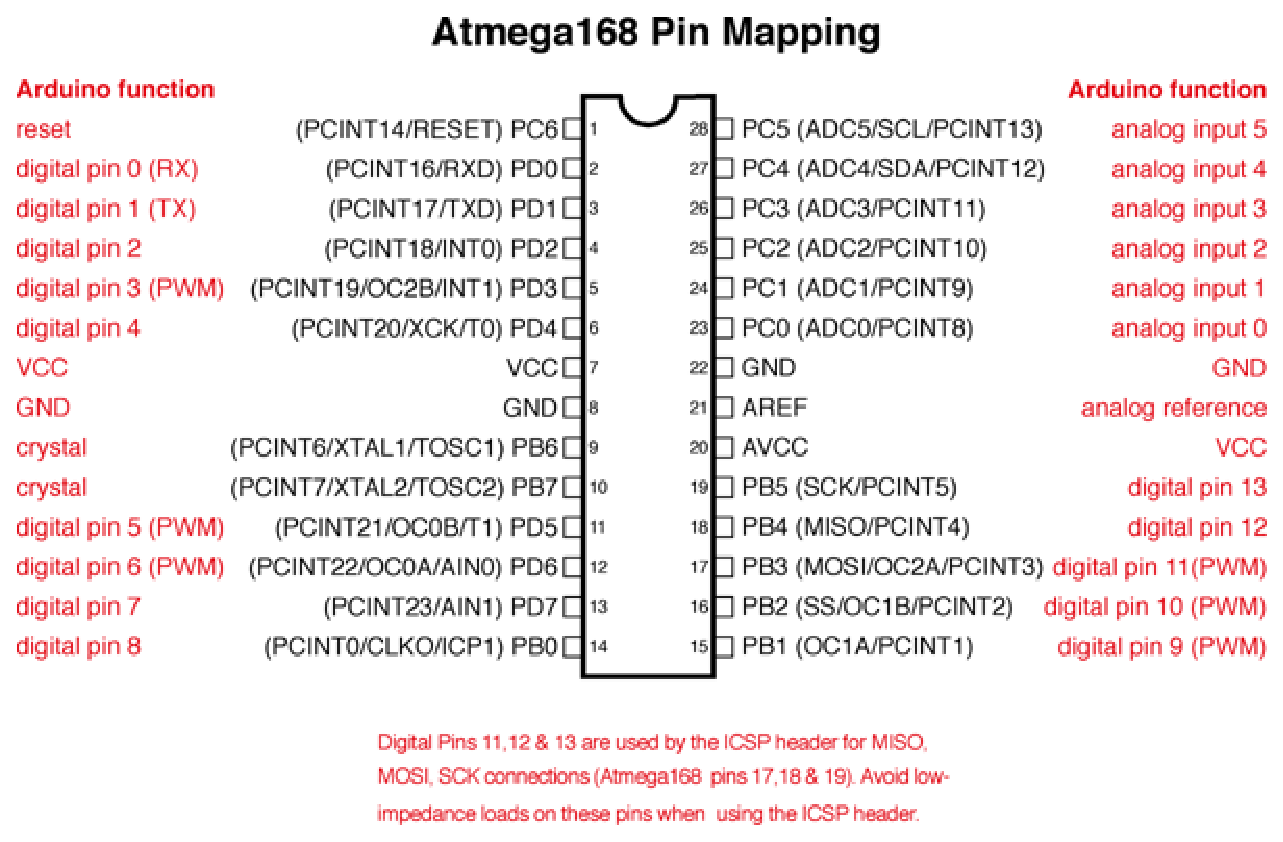
\includegraphics[width=0.8\textwidth]{pins}
    \caption{Pinout for ATMEGA168/328 DIP package} 
    \label{fig:pins}
    \end{centering}
\end{figure}




\centering
\vspace{2cm}
\appendix

\end{document}

